\documentclass[tikz, border = 10pt]{standalone}


\usepackage{newpxtext,newpxmath}   % /upbeta
%\usepackage{fouriernc}            % /otherbeta
\usepackage{amsmath}
\renewcommand{\familydefault}{\sfdefault}
\usepackage{mathastext}

\usetikzlibrary{positioning, quotes, calc, math, arrows.meta, bending, shapes, backgrounds}

\tikzset{
every edge quotes/.style = {fill = white},
every node/.style = {scale = 1.1},
manifest/.style = {rectangle, draw, thin, inner sep = 3pt, minimum width = 1cm,
   minimum height = .85cm, align = center},
latent/.style = {ellipse, draw, thin, inner sep = 3pt, minimum width = 1cm,
   minimum height = .85cm},
residual1/.style = {circle, draw, thin, minimum size = 5mm, inner sep = 1pt},
residual2/.style = {rectangle, minimum width = 0.5pt, minimum height = 1.5mm,
   inner sep = 0pt, outer sep = 0mm},
regression/.style = {-{Stealth[length = 1.5mm]}, thin, shorten > = 1pt, 
   inner sep = 1.5pt, outer sep = 0mm},
covariance/.style={{Stealth[length = 1.5mm]}-{Stealth[length = 1.5mm]}, thin,
   shorten > = 1pt, shorten < = 1pt, inner sep = 1.5pt},
variance/.style={{Stealth[length = 1mm]}-{Stealth[length = 1mm]}, thin,
   shorten > = 1pt, shorten < = 1pt, inner sep = 1pt},
interaction/.style = {-{Stealth[sep = 1pt, length = 1.5mm] . Circle[length = 4pt]},
   thin, shorten > = -2pt},
constant/.style = {draw, thin, inner sep = 1pt, regular polygon,
   regular polygon sides = 3, minimum size = 5mm},
group/.style = {rectangle, inner sep = 2pt, minimum width = 15mm, minimum height = 5mm, 
   align = center}
}
\usetikzlibrary{matrix}

\begin{document}
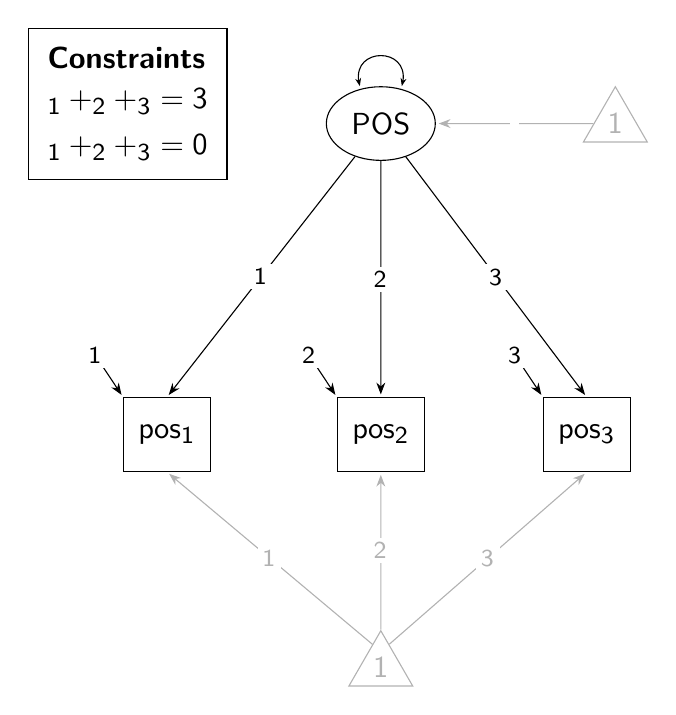
\begin{tikzpicture}

%% pos manifests
\node [manifest] (pos1) {$pos_1$};
\node [manifest] (pos2) [right = 1.6cm of pos1] {$pos_2$};
\node [manifest] (pos3) [right = 1.5cm of pos2] {$pos_3$};

%% POS latent
\node [latent] (POS) [above = 3cm of pos2] {$POS$};

%% Loadings
\path [regression] (POS) edge ["$\uplambda_1$"] (pos1.90);
\path [regression] (POS) edge ["$\uplambda_2$"] (pos2.90);
\path [regression] (POS) edge ["$\uplambda_3$"] (pos3.90);

%% Latent variance
\path [variance] (POS.120) edge ["$\upphi$", above, outer sep = 1pt, bend left = 110, looseness = 3] (POS.60);

%% Residuals
\node [residual2] (e1) [above left = .65cm of pos1, xshift = 1mm] {};
\path [regression] (e1) edge ["$\uptheta_1$", pos = 0] (pos1.north west);

\node [residual2] (e2) [above left = .65cm of pos2, xshift = 1mm] {};
\path [regression] (e2) edge ["$\uptheta_2$", pos = 0] (pos2.north west);

\node [residual2] (e3) [above left = .65cm of pos3, xshift = 1mm] {};
\path [regression] (e3) edge ["$\uptheta_3$", pos = 0] (pos3.north west);

%% latent means
\node [constant, black!30] (M1) [right = 2cm of POS] {1};
\node [constant, black!30] (M2) [below = 2cm of pos2] {1};
\path [regression, black!30] (M1) edge ["$\upkappa$"] (POS);

%% Intercepts
\path [regression, black!30] (M2.110) edge ["$\uptau_1$"] (pos1.270);
\path [regression, black!30] (M2.90) edge ["$\uptau_2$"] (pos2.270);
\path [regression, black!30] (M2.70) edge ["$\uptau_3$"] (pos3.270);

\matrix [matrix of nodes, draw, cells = {anchor = west}] at (-0.5, 4.2) {
   \bf{Constraints}\\
   $\uplambda_1 + \uplambda_2 + \uplambda_3 = 3$ \\ 
   $\uptau_1 + \uptau_2 + \uptau_3 = 0$ \\
};

\end{tikzpicture}
\end{document}

